\documentclass{article}
\usepackage[english]{babel}
\usepackage[utf8]{inputenc}
\usepackage{multirow}
\usepackage{booktabs}
\usepackage{mathtools}
\usepackage{amsmath}
\usepackage{amsfonts}
\usepackage{amssymb}
\usepackage{graphicx}
\usepackage[skip=10pt]{caption}
\usepackage{subcaption}
\usepackage{float}
\usepackage{rotating}
\usepackage{array}
\usepackage{enumitem}
\addtolength{\oddsidemargin}{-.875in}
\addtolength{\evensidemargin}{-.875in}
\addtolength{\textwidth}{1.75in}
\addtolength{\topmargin}{-.875in}
\addtolength{\textheight}{1.75in}
\usepackage{fancyhdr}
\usepackage{xcolor}
\usepackage{algorithm}
\usepackage[noend]{algpseudocode}
%\usepackage[linesnumbered,ruled]{algorithm2e}
\usepackage[framemethod=default]{mdframed}
\newmdenv[linecolor=black,backgroundcolor=cyan!10]{algo}
\newmdenv[linecolor=black,backgroundcolor=gray!10]{algo2}
\newmdenv[linecolor=gray!20,backgroundcolor=gray!20]{biomathg}
\newmdenv[linecolor=black!30,backgroundcolor=red!20]{biomathr}
\newmdenv[linecolor=black!30,backgroundcolor=yellow!20]{biomathy}
\newmdenv[linecolor=black!30,backgroundcolor=blue!5]{biomathb}
\newmdenv[linecolor=black,backgroundcolor=cyan!10]{biomathc}
\usepackage{listings}

 \lstset{
  language=R,                     % the language of the code
  basicstyle=\ttfamily,       % the size of the fonts that are used for the code
  numbers=none,                   % where to put the line-numbers
  %backgroundcolor=\color{lightgray},  % choose the background color. You must
                                % add \usepackage{color}
  columns=fullflexible,
  showspaces=false,               % show spaces adding particular underscores
  showstringspaces=false,         % underline spaces within string
  showtabs=false,                 % show tabs within strings adding particular underscores
  tabsize=2,                      % sets default tabsize to 2 spaces
  breaklines=true,                % sets automatic line breaking
  keywordstyle=\color{blue},      % keyword style
  commentstyle=\color{darkgray},   % comment style
  stringstyle=\color{red},      % string literal style
  alsoletter={._},
  %otherkeywords={!,!=,~,$,\&,\%/\%,\%*\%,\%\%,<-,<<-}
}

\newcounter{subfloat}
\renewcommand{\thesubfloat}{\alph{subfloat}}
\newcommand{\image}[2]{%
  \stepcounter{subfloat}%
  \begin{tabular}[t]{@{}c@{}}
  #2 \\
  (\thesubfloat) #1
  \end{tabular}%
}







\begin{document}

\begin{center}

%  \textsc{\huge University of Ottawa} \\
  \vspace{1cm}
  
\includegraphics[scale = 0.8]{uottawa_hor_black.png}
  \vspace*{3.5cm}



  \begin{minipage}{0.9\textwidth} 
    \begin{center}
      \textsc{\LARGE Final Project - Part 1 Option B}
    \end{center}
  \end{minipage}\\[0.5cm]
  
  \vspace*{1cm}

  { \huge \bfseries  Handwritten Digit Recognition with Neural Networks}

  \vspace*{2cm}
  { \large 
      \emph{Team:} PACmen \\
      \vspace*{1cm}
    \emph{Members:}\\	
      Soufiane Fadel (300089065) \\
      Zhibin Liu (300056998) \\
      Loïc Muhirwa (300090370)\\
      Scott Parkinson (300063940)\\
      Alexandre Ren\'e (5008305) \\
      Ezekiel Williams (5858100)\\
    \vspace*{2.5cm}
    \emph{Professor:} \\													  
    Dr. Maia Fraser \\
  }
    \vspace{2cm}
    MATH 5314C (Winter 2019)	\\
    \vspace{1cm}
  \begin{center}
    {April 26, 2019}
  \end{center}
  
\end{center}
																		
\newpage	







\begin{center}
\textbf{Part 0 }
\end{center}

For this project we are asked to use the classic MNIST data set. The data set is comprised of size normalized and centered 28x28 pixel gray scale images of handwritten digits 0 to 9. The set is comprised of 60,000 training images and a test set with 10,000 images. The MNIST data set is modified version of the NIST data set and is widely used for machine learning testing and development. 

We first construct an accessor class for the MNIST data which concatenates the training and test samples, and for each assembles the ground truth labels in both sparse and one-hot output vectors.

\vspace{0.5cm}

\begin{biomathy}
\begin{lstlisting}[language=python]
class MNIST:
    """
    x_train: concatenated training data sets
             Dimensions are (N,M), where N: feature size, M: no. of samples
    x_test:  concatenated test data sets
             Dimensions are (N',M'), where N': feature size, M': no. of samples
    y_train: 1-D vector of length M
    y_test:  1-D vector of length M'
    y_mat_train:  1-hot matrix of training labels. NxM
    y_mat_test:   1-hot matrix of test labels. NxM'
    """
    labels = "0 1 2 3 4 5 6 7 8 9".split(' ')
    data_shape = (28**2,)
    nlabels = len(labels)

    def __init__(self, filename):
        self.data = load(filename, sio.loadmat)
        # Data values are between 0-255; normalize them to 0-1
        for k, v in self.data.items():
            if 'train' in k or 'test' in k:
                self.data[k] = v / 255.0
        # Create concatenated data sets
        self.x_train = np.vstack([D for D in self.train_data]).T
        self.x_test = np.vstack([D for D in self.test_data]).T
        self.y_train = np.concatenate(
            [[i]*D.shape[0] for i, D in enumerate(self.train_data)] )
        self.y_test = np.concatenate(
            [[i]*D.shape[0] for i, D in enumerate(self.test_data)] )
        k = len(self.labels)
        M, Mp = len(self.y_train), len(self.y_test)
        self.y_mat_train = np.zeros((k, M), dtype=np.float)
        self.y_mat_test = np.zeros((k, Mp), dtype=np.float)
            # Must be a real type for gradient descent
        for i, y in enumerate(self.y_train):
            self.y_mat_train[y, i] = 1
        for i, y in enumerate(self.y_test):
            self.y_mat_test[y, i] = 1

    def __len__(self):
        return len(self.y_train)

    @property
    def train_data(self):
        """Returns a generator expression for the training data.
           Guaranteed to be in the order 0,1,...,9.
        """
        return (self.data['train{}'.format(i)] for i in range(10))
    @property
    def test_data(self):
        """Returns a generator expression for the training data."""
        return (self.data['test{}'.format(i)] for i in range(10))
\end{lstlisting}
\end{biomathy}


\vspace{1cm}


\begin{center}
\textbf{Part 1 }
\end{center}

\begin{biomathg}
Plotting  the 10 images of each of the digits.
\end{biomathg}
\vspace{0.5cm}


\noindent The data is sourced from the mnist\_all.mat  file and the code to generate this is given as follows using matplotlib and subplot to  sample 10 images of each digit: \\

\noindent \underline{\textbf{Python code:}} \\
\begin{biomathy}
\begin{lstlisting}[language=python]
def plot_data_samples(MNIST, fig=None):
    if fig is None: fig = plt.fig()
    img_indices = np.random.random_integers(0, 5000, 10)
    ax = fig.subplots(10,10)

    for i in range(10):
        for j in range(10):
            ax[i,j].imshow(MNIST["train"+str(i)][img_indices[j]].reshape((28,28)))
            ax[i,j].axis('off')
    return fig, ax

data = MNIST('mnist_all.mat')
fig1 = plt.figure(figsize=(7,7))
fig1, ax = plot_data_samples(data.data, fig=fig1)
\end{lstlisting}
\end{biomathy}

\pagebreak
\noindent \underline{\textbf{Output:}} \\


\begin{figure}[H]
        \centering
        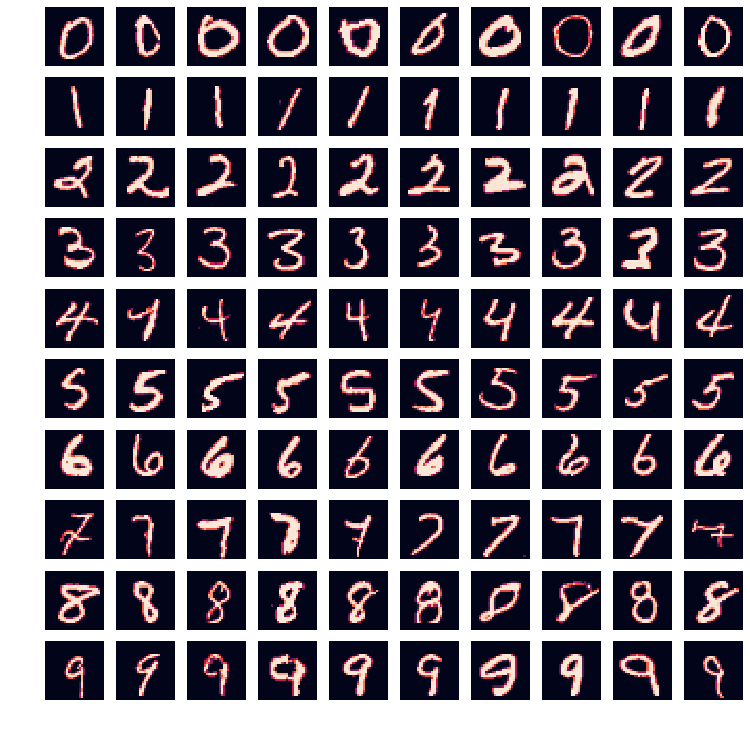
\includegraphics{fig1.pdf}
        \caption{10 images of each of the digits (fig1.pdf).}
        \label{fig1}
\end{figure}

\pagebreak
\begin{center}
\textbf{Part 2 }
\end{center}
\begin{biomathg}
Implementation of the  \textbf{softmax} and \textbf{forward}   functions.
\end{biomathg}
%\begin{figure}[H]
%        \centering
%        \includegraphics[scale = 0.6 ]{figp2.png}
%\end{figure}

\vspace{1cm}



\noindent The form of the softmax function is given by:
$ \forall  1 \leq t  \leq m = 60000 \text{ and } 1 \leq i  \leq 10$ :
\begin{align*}
(\textbf{softmax}(o^{(t)}))_i = \frac{e^{o^{(t)}_{i}}}{\sum_{k=1}^{10}e^{o^{(t)}_{k}}}
\end{align*}

\noindent and the forward function for one training example is:
$$\textbf{forward}(w,b,x) = w^{t}x +b $$

\noindent In our code we calculate the forward function for the whole training set.
\\ \\
\noindent \underline{\textbf{Python code:}} \\
\begin{biomathy}
\begin{lstlisting}[language=python]
def softmax(o):
    return np.exp(o)/sum(np.exp(o))

def forward(W, x, b):
    B = np.tile(b, x.shape[1])
    o = np.dot(W.T, x) + B
    P = np.zeros((10,x.shape[1]))
    for i in range(x.shape[1]):
        P[:,i] = softmax(o[:,i])
    return P
\end{lstlisting}
\end{biomathy}

\pagebreak
\begin{center}
\textbf{Part 3 }
\end{center}


\begin{biomathg}
 Gradient descent calculation
\end{biomathg}

\vspace{0.3cm}

\noindent Our goal here is  using gradient descent to  minimize  the negative  log-probabilities cost function $C(w)$ of the correct answer for the N training cases under consideration as the cost function. 
\begin{align*}
\underset{w \in \mathbb{R}^{784\times m}}{\min} \left\{
-\sum_{t=1}^{m}\sum_{k=1}^{10} y_{k}^{(t)}\log\left( p_{k}^{(t)}\right)
\right\}
\end{align*}
\text{where,}
$ \text{for all } 1 \leq t  \leq m = \#\{\text{training set}\}, 1 \leq i  \leq 10$ :
\begin{align*}
o_i^{(t)} &= \sum_{k=1}^{784}w_{k,i}x_{k}^{(t)} + b_i \\
p^{(t)}_{i} &=(\textit{softmax}(o^{(t)}))_i = \frac{e^{o^{(t)}_{i}}}{\sum_{k=1}^{10}e^{o^{(t)}_{k}}}
\end{align*}
The minimization will be done with the gradient descent algorithm that require calculation of the partial derivative $\frac{\partial C}{\partial w_{ij}}$ which can be expressed as  follows (using chain rule)

\begin{align*}
\frac{\partial C}{\partial w_{ij}} =&\frac{\partial C}{\partial p^{(t)}_{k}}
\frac{\partial  p^{(t)}_{k}}{\partial o^{(t)}_{j}}
\frac{\partial  o^{(t)}_{j}}{\partial w_{ij}}\\
=&- \sum_{t=1}^{m}\sum_{k=1}^{10}
\frac{y^{(t)}_{k}}{ p^{(t)}_{k}}
\frac{\partial  p^{(t)}_{k}}{\partial o^{(t)}_{j}}
\frac{\partial  o^{(t)}_{j}}{\partial w_{ij}} \\
\end{align*}

let's now calculate $\frac{\partial  p^{(t)}_{k}}{\partial o^{(t)}_{j}}$ and
$\frac{\partial  o^{(t)}_{j}}{\partial w_{ij}}$ separately.

\begin{itemize}
\item[•]\textbf{ the term $\frac{\partial  p^{(t)}_{k}}{\partial o^{(t)}_{j}}$ : }
\begin{align*}
\frac{\partial  p^{(t)}_{k}}{\partial o^{(t)}_{j}} &= \frac{\partial \left[ \frac{e^{o^{(t)}_{k}}}{\sum_{k=1}^{10}e^{o^{(t)}_{k}}} \right] }{\partial o^{(t)}_{j}}\\
=&
\begin{cases}
\frac{
e^{o^{(t)}_{j}}\left[\sum_{k=1}^{10}e^{o^{(t)}_{k}}\right] - e^{o^{(t)}_{j}}e^{o^{(t)}_{j}}
}{\left[\sum_{k=1}^{10}e^{o^{(t)}_{k}}\right]^2}
& \text{ if } j=k \\
\frac{ - e^{o^{(t)}_{k}}e^{o^{(t)}_{j}}
}{\left[\sum_{k=1}^{10}e^{o^{(t)}_{k}}\right]^2}
& \text{ if } j \neq k
\end{cases}\\
=&
\begin{cases}
p^{(t)}_{j}(1-p^{(t)}_{j})
& \text{ if } j=k \\
-p^{(t)}_{j}p^{(t)}_{k}
& \text{ if } j \neq k
\end{cases}
\end{align*}
\item[•]\textbf{ the term $\frac{\partial  o^{(t)}_{j}}{\partial w_{ij}}$ : }
\begin{align*}
\frac{\partial  o^{(t)}_{j}}{\partial w_{ij}} &= \frac{\partial  \left[
\sum_{k=1}^{784}w_{k,j}x_{k}^{(t)} + b_j \right]}{\partial w_{ij}}  \\
&= x_{i}^{(t)}
\end{align*}
\end{itemize}
By grouping  all the  terms we have :

\begin{align*}
\frac{\partial C}{\partial w_{ij}} =& - \sum_{t=1}^{m}\sum_{k=1}^{10}
\frac{y^{(t)}_{k}}{ p^{(t)}_{k}}
\frac{\partial  p^{(t)}_{k}}{\partial o^{(t)}_{j}}
\frac{\partial  o^{(t)}_{j}}{\partial w_{ij}} \\
&= - \sum_{t=1}^{m}\left[
\frac{y^{(t)}_{j}}{ p^{(t)}_{j}}
\frac{\partial  p^{(t)}_{j}}{\partial o^{(t)}_{j}}
\frac{\partial  o^{(t)}_{j}}{\partial w_{ij}}
+
\sum_{k \neq j }^{10}
\frac{y^{(t)}_{k}}{ p^{(t)}_{k}}
\frac{\partial  p^{(t)}_{k}}{\partial o^{(t)}_{j}}
\frac{\partial  o^{(t)}_{j}}{\partial w_{ij}}
\right]
\\
&= - \sum_{t=1}^{m}\left[
\frac{y^{(t)}_{j}}{ p^{(t)}_{j}} p^{(t)}_{j}(1-p^{(t)}_{j}) x_{i}^{(t)}
+ \sum_{k \neq j }^{10} -\frac{y^{(t)}_{k}}{ p^{(t)}_{k}} p^{(t)}_{j}p^{(t)}_{k} x_{i}^{(t)} \right] \\
&= - \sum_{t=1}^{m}\left[ \left(  y^{(t)}_{j}(1-p^{(t)}_{j})
+ \sum_{k \neq j }^{10} - y^{(t)}_{k} p^{(t)}_{j} \right)x_{i}^{(t)} \right] \\
&= - \sum_{t=1}^{m}\left[ \left( y^{(t)}_{j}- \sum_{k = 1 }^{10} y^{(t)}_{k}p^{(t)}_{j}\right) x_{i}^{(t)} \right]
\\
&= - \sum_{t=1}^{m}\left[ \left(  y^{(t)}_{j}(1-p^{(t)}_{j})
+\sum_{k \neq j }^{10} - y^{(t)}_{k} p^{(t)}_{j} \right)x_{i}^{(t)} \right] \\
&= - \sum_{t=1}^{m}  \left( y^{(t)}_{j} - p^{(t)}_{j} \right) x_{i}^{(t)}
\hspace{3cm} \left(\sum_{k = 1 }^{10}
 y^{(t)}_{k} =1 \right) \\
&= \sum_{t=1}^{m}  \left( p^{(t)}_{j}-y^{(t)}_{j} \right)x_{i}^{(t)}
\end{align*}

Similarly since :

\begin{align*}
\frac{\partial  o^{(t)}_{j}}{\partial b_{j}} &= \frac{\partial  \left[
\sum_{k=1}^{784}w_{k,j}x_{k}^{(t)} + b_j \right]}{\partial b_{j}}  \\
&= 1
\end{align*}
then we have :


\begin{align*}
\frac{\partial C}{\partial b_{j}} =& - \sum_{t=1}^{m}\sum_{k=1}^{10}
\frac{y^{(t)}_{k}}{ p^{(t)}_{k}}
\frac{\partial  p^{(t)}_{k}}{\partial o^{(t)}_{j}}
\frac{\partial  o^{(t)}_{j}}{\partial b_{j}} \\
&= \vdots \ \ \ \vdots \ \ \ \vdots \ \ \ \vdots  \\
&= \sum_{t=1}^{m}  \left(p^{(t)}_{j}-y^{(t)}_{j}\right)
\end{align*}

\noindent \underline{\textbf{the  vectorisation of the  solution:}} \\ \\
\noindent The last form  of gradient  can be expressed  as:
\begin{align*}
\begin{cases}
\nabla_w C = (P-Y)X^{t}  \\
\nabla_b C = (P-Y)\mathbb{1}
\end{cases}
\end{align*}

where :
\begin{align*}
\nabla_w C =& \left(\frac{\partial C}{ \partial w_{i,j}} \right)_{i,j}
= \begin{bmatrix}
    \frac{\partial C}{ \partial w_{1,1}} & \frac{\partial C}{ \partial w_{1,2}} &\cdots & \frac{\partial C}{ \partial w_{1,784}}   \\
  \frac{\partial C}{ \partial w_{2,1}} & \frac{\partial C}{ \partial w_{2,2}} &\cdots & \frac{\partial C}{ \partial w_{2,784}}   \\
  \vdots & \vdots & \ddots  & \vdots \\
  \frac{\partial C}{ \partial w_{10,1}} & \frac{\partial C}{ \partial w_{10,2}} &\cdots & \frac{\partial C}{ \partial w_{10,784}}   \\
  \end{bmatrix}  \\
 P =& \left(p_i^{(t)} \right)_{i,t} =
\begin{bmatrix}
   p_1^{(1)} & p_1^{(2)}  &\cdots &  p_1^{(m)}  \\
   p_2^{(1)} & p_2^{(2)}  &\cdots &  p_2^{(m)}  \\
  \vdots & \vdots & \ddots  & \vdots \\
   p_{10}^{(1)} & p_{10}^{(2)}  &\cdots &  p_{10}^{(m)}  \\
  \end{bmatrix}  \\
   X =& \left(x_i^{(t)} \right)_{i,t} =
\begin{bmatrix}
   x_1^{(1)} & x_1^{(2)}  &\cdots &  x_1^{(m)}  \\
   x_2^{(1)} & x_2^{(2)}  &\cdots &  x_2^{(m)}  \\
  \vdots & \vdots & \ddots  & \vdots \\
   x_{784}^{(1)} & x_{784}^{(2)}  &\cdots &  x_{784}^{(m)}
  \end{bmatrix} \\
  Y =& \left(y_i^{(t)} \right)_{i,t} =
\begin{bmatrix}
   y_1^{(1)} & y_1^{(2)}  &\cdots &  y_1^{(m)}  \\
   y_2^{(1)} & y_2^{(2)}  &\cdots &  y_2^{(m)}  \\
  \vdots & \vdots & \ddots  & \vdots \\
   y_{10}^{(1)} & y_{10}^{(2)}  &\cdots &  y_{10}^{(m)}
  \end{bmatrix} \\
   \mathbb{1} =& \begin{bmatrix} 1 \\ 1 \\ \vdots \\ 1 \end{bmatrix}
\end{align*}

Furthermore, we also give the function of the negative-log loss function:

$$\textbf{Neg\_Log\_proba}(w,x,y) = \sum_{i=0}^{9}y^t_i\log(p^t_i) $$


\noindent \underline{\textbf{Python code:}} \\
\begin{biomathy}
\begin{lstlisting}[language=python]
def Neg_Log_proba(W,x_train,b, y_train):
    return -np.sum(y_train*np.log(forward(W, x_train, b)))

def gradient(X, Y, W, b):
   N = 10
   P = forward(W, X, b)
   dO = P - Y
   dW = np.dot(X, dO.T)
   db = np.sum(dO, 1).reshape(N, 1)
   return dW, db
\end{lstlisting}
\end{biomathy}


\pagebreak
\begin{center}
\textbf{Part 4 }
\end{center}
\begin{biomathg}
 Check  the  gradient  algorithm
\end{biomathg}

\vspace{0.5cm}

\noindent In order to verify that our  computation of  the gradient in Part 3 is correct we are using a finite-difference approximation for several coordinates of $W$  an d $b$.  
\noindent Mathematically the finite differences methods is given by:
$$\frac{\partial C}{\partial w} = \lim_{h\rightarrow 0}\frac{C(w+h)-C(w)}{h} $$

 \noindent So in order to check   our gradient  algorithm, we shall try to calculate the quantity $\left(\frac{\partial C}{\partial w} \right)_{i,j} \approx \frac{C(w_{i,j}+h)-C(w)}{h} $  for
 different component $(i,j)$ and   a small $h$ and then compare it  to our gradient algorithm value.  \\

\noindent \underline{\textbf{Python code:}} \\
\begin{biomathy}
\begin{lstlisting}[language=python ]
def gradient_finite_diff(x_train, y_train , W, b, i, j, h=1e-7):
    deltaij = np.zeros(W.shape)
    deltaij[i, j] = h

    cost   = Neg_Log_proba(W,x_train,b, y_train)
    cost_h = Neg_Log_proba(W+deltaij,x_train,b, y_train)

    return (cost_h - cost)/h

samples_i = [288, 600, 100]
samples_j = [8, 4, 1]
for i, j in zip(samples_i, samples_j):
    W = np.random.uniform(0, 1, (28*28, 10))
    b = np.random.uniform(0,1,(10, 1))
    gf = gradient_finite_diff(data.x_train, data.y_mat_train, W, b, i, j)
    g = gradient(data.x_train, data.y_mat_train, W, b)[0][i, j]
    print('W[{:d}, {:d}]'.format(i, j))
    print('--------------------------------------')
    print('grad_dWij: {:.7f}\nfinite-difference approximation: {:.7f}'
          .format(g, gf))
    print('absolute difference: {:.7f}\n'.format(abs(g - gf)))
\end{lstlisting}
\end{biomathy}
\pagebreak
\noindent \underline{\textbf{Output:}} \\


% TODO: Update with final run
\begin{biomathc}
\begin{lstlisting}[language=python]
W[288, 8]
--------------------------------------
grad_dWij: 1422.6502531
finite-difference approximation: 1422.6505300
absolute difference: 0.0002769

W[600, 4]
--------------------------------------
grad_dWij: -78.6249408
finite-difference approximation: -78.6251621
absolute difference: 0.0002214

W[100, 1]
--------------------------------------
grad_dWij: 331.3443073
finite-difference approximation: 331.3444904
absolute difference: 0.0001831
\end{lstlisting}
\end{biomathc}


\pagebreak
\begin{center}
\textbf{Part 5 }
\end{center}

%TODO: Update numbers
\begin{biomathg}
Training the linear neural network.
\end{biomathg}

\vspace{0.5cm}


\noindent Our  neural  network is optimised  by  mini-batch gradient descent.  The performance was tested for a learning rate of  $0.01$ and a batch sizes of $50$ and  as it's shown below in the learning curve converged very quickly just after 35 iterations  with an accuracy of $92 \%$.\\
The examples of correctly and incorrectly classified samples are given in Figures \ref{fig2a} and \ref{fig2b} respectively (See supplementary python file for the complete code).
\vspace{0.5cm}

\noindent \underline{\textbf{Python code:}} \\
\begin{biomathy}
\begin{lstlisting}[language=python]
def accuracy(x, w, b, y):
    corr = 0
    output = forward(w, x, b)
    for i in range(y.shape[1]):
        if (y[np.argmax(output[:, i]), i] == 1):
            corr += 1
    return corr/float(y.shape[1])

def train_nn(x_train, y_train, x_test, y_test,  max_it = 35):

    c = load("LNN_fit_cache_{}.npz".format(max_it), np.load)
    if c is not None:
        # Return previous fit from disk cache
        return (c['W'], c['b'], c['itera'],
                c['train_accuracy'], c['test_accuracy'],
                c['train_costs'], c['test_costs'])

    itera , train_accuracy, test_accuracy = [], [], []
    train_costs , test_costs = [], []

    init_W = np.zeros((28*28, 10))
    init_b = np.zeros((10, 1))

    W = init_W.copy()
    b = init_b.copy()
    alpha = 0.01
    batch_size = 50

    for t in range(max_it):
        indices = np.random.permutation(x_train.shape[1])
        x_train = x_train[:,indices]
        y_train = y_train[:,indices]

        for it in range(0, x_train.shape[1], batch_size):
            x_train_i = x_train[:,it:it+batch_size]
            y_train_i = y_train[:,it:it+batch_size]

            dW, db =  gradient(x_train_i, y_train_i, W, b)
            W = W  -  alpha/batch_size * dW
            b = b  -  alpha/batch_size * db


        train_accuracy_i = accuracy(x_train, W, b, y_train)
        test_accuracy_i = accuracy(x_test, W, b, y_test)
        train_cost_i = Neg_Log_proba(W,x_train,b, y_train)
        test_cost_i = Neg_Log_proba(W,x_test,b, y_test)

        itera.append(t)
        train_accuracy.append(train_accuracy_i)
        test_accuracy.append(test_accuracy_i)
        train_costs.append(train_cost_i)
        test_costs.append(test_cost_i)

        print("itreration: " + str(t))
        print("Training Performance:   " + str(train_accuracy_i) + "%")
        print("Testing Performance:    " + str(test_accuracy_i) + "%")
        print("Training cost:   " + str(train_cost_i) )
        print("Testing cost:    " + str(test_cost_i) + "\n")

        # Terminate if there is no more gain on the test set
        if len(test_accuracy) > 2:
            train_diff = (train_accuracy[-1] - train_accuracy[-2])/train_accuracy[-1]
            test_diff = (test_accuracy[-1] - test_accuracy[-2])/test_accuracy[-1]
            if train_diff < 0.001 and test_diff < 0.001:
                break

    np.savez("LNN_fit_cache_{}.npz".format(max_it), W=W, b=b, itera=itera,
             train_accuracy=train_accuracy, test_accuracy=test_accuracy,
             train_costs=train_costs, test_costs=test_costs)
    return W, b, itera, train_accuracy, test_accuracy, train_costs, test_costs

W, b, epochs, train_accuracy, test_accuracy, train_costs, test_costs \
    = train_nn(data.x_train, data.y_mat_train,
               data.x_test, data.y_mat_test, max_it = 35)
\end{lstlisting}
\end{biomathy}



\noindent \underline{\textbf{Output:}} \\


\begin{figure}[H]
        \centering
        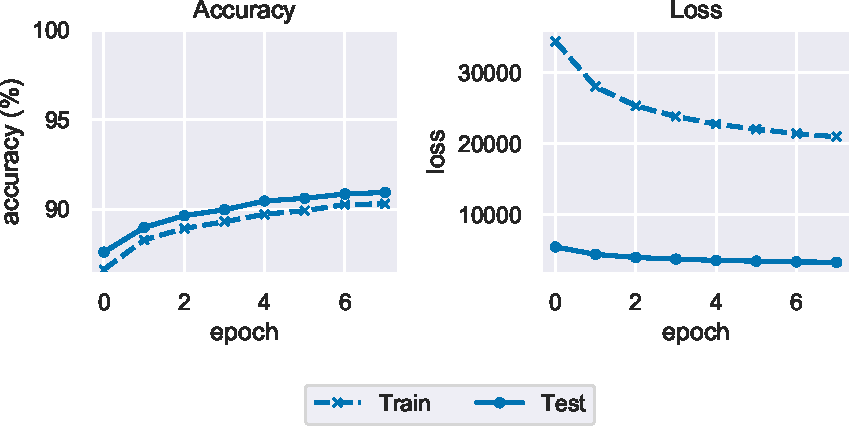
\includegraphics{fig3.pdf}
        \caption{Loss and accuracy learning curves for the linear neural
        network (fig3.pdf).}
        \label{fig3}
\end{figure}


\begin{figure}[H]
        \centering
        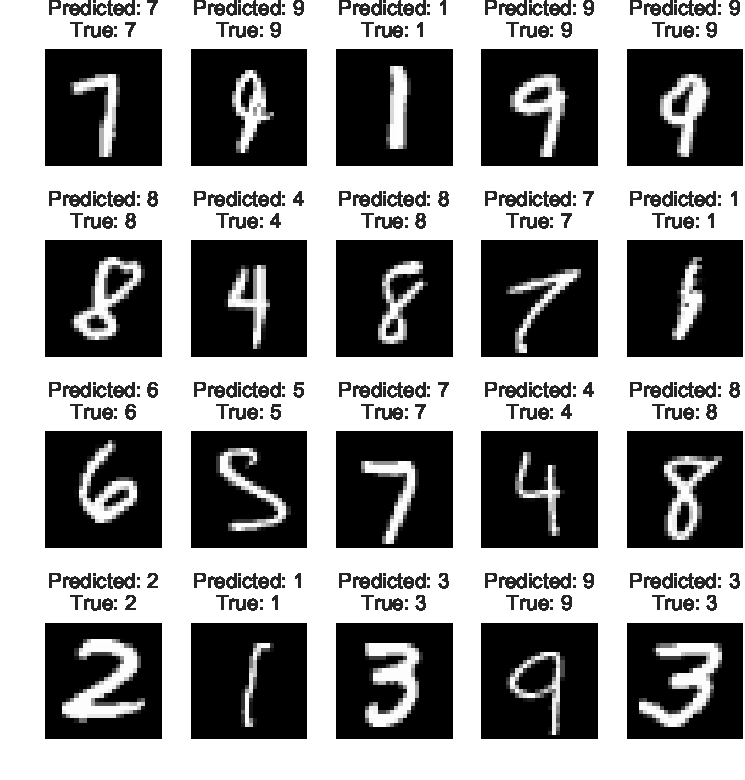
\includegraphics{fig2a.pdf}
        \caption[width=7in]{Random selection of correctly classified MNIST numbers from the test set (fig2a.pdf).}
        \label{fig2a}
\end{figure}

\noindent \\
\begin{figure}[H]
        \centering
        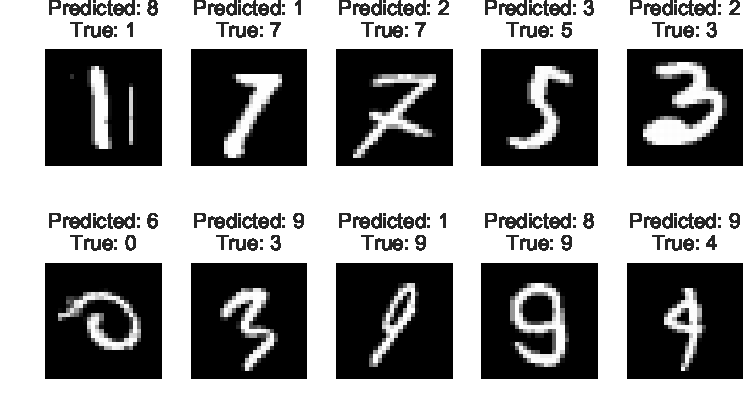
\includegraphics{fig2b.pdf}
        \caption[width=7in]{Random selection of incorrectly classified MNIST numbers from the test set (fig2b.pdf).}
        \label{fig2b}
\end{figure}

\pagebreak
\begin{center}
\textbf{Part 6 }
\end{center}


\begin{biomathg}
Weight visualisation.
\end{biomathg}

\vspace{0.5cm}

 %\noindent Visualizing  each of the set of W's that connect to $o_0$, the set of W's that connect to $o_1$, etc, with each $w_ji$ displayed at an appropriate pixel.

\noindent  In this question we are  visualizing each of the set of W's that connect to each of the output digits. The weights connecting to each output are visualized below and we see clearly the pattern of the handwritten digits for each case.  \\

\noindent \underline{\textbf{Python code:}} \\
\begin{biomathy}
\begin{lstlisting}[language=python]
def visualize_unit_weights(weights, units, maxcols=4, fig=None, LNN=False):
    """
    weights: Iterable of all weight matrices corresponding to the units.
    units:   Indices of the units for which we want to print the weights.
    maxcols: Number of columns in the output. Default: 4.
    fig:     If provided, axes on drawn on this figure.
    LNN:     Bool. Changes figure title for the LNN.
    """

    if fig is None: fig = plt.figure()
    ncols = min(len(units), maxcols)
    nrows = np.ceil(len(units) / ncols).astype(int)
    gs = GridSpec(nrows, ncols+1,
                  width_ratios= [1]*ncols + [ncols/20])
    cax = fig.add_subplot(gs[:, -1])  # Colorbar axes
    # Ensure all plots use same colour scale
    vmax = max(weights[:,u].max() for u in units)
    vmin = max(weights[:,u].min() for u in units)
    axes = []
    for i, u in enumerate(units):
        w = weights[:, u].reshape(28, 28)
        ax = fig.add_subplot(gs[i + i//ncols])
        if LNN:
            ax.set_title("Weights for {}".format(u))
        else:
            ax.set_title('Weights to unit {}'.format(u+1))
        cbar=(i==len(units)-1)  # Only print colorbar on the last axes
        if sns:
            sns.heatmap(w, vmin=vmin, vmax=vmax, cmap='coolwarm', cbar_ax=cax)
        else:
            print("Seaborn required for weight matrix visualizatons.")
        ax.axis('off')
        axes.append(ax)
    return fig, axes, cax

visualize_unit_weights(W, range(10), maxcols=3, LNN=True, fig=fig4)
\end{lstlisting}
\end{biomathy}

\begin{figure}[H]
        \centering
        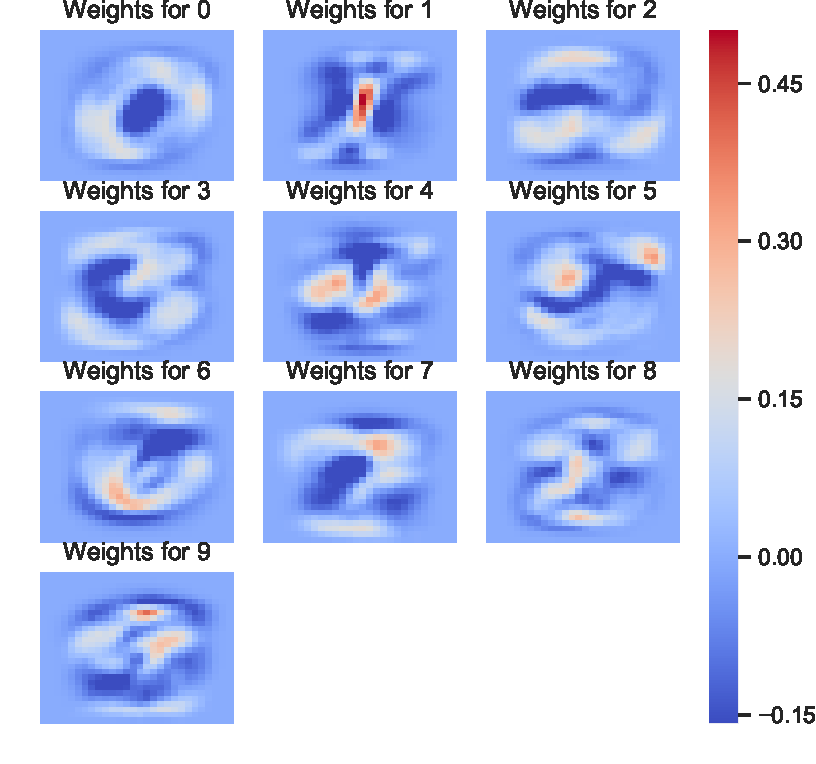
\includegraphics{fig4.pdf}
        \caption[width=7in]{Readout units show a weight distribution reminiscent of the digit to which they correspond (fig4.pdf).}
\end{figure}




\pagebreak
\begin{center}
\textbf{Part 7 }
\end{center}
\begin{biomathg}
\noindent Implementation of Feed-forward Neural Network (FNN)
\end{biomathg}
%\begin{figure}[H]
%        \centering
%        \includegraphics[scale = 0.6]{figp7.png}
%\end{figure}
\vspace{0.5cm}
To perform a more thorough classification of the data set we implemented a standard FNN with nonlinear activations; specifically, we used Keras' \texttt{Sequential} model. This FNN had one hidden layer with tanh activation functions; softmax was used on the output layer. We implemented two versions of this network, the second including an additional dropout layer for regularization. Tanh activation functions were employed in the hidden layer while softmax was used in the output layer. Full network parameters are given in Table \ref{ztable1}, alongside the parameters for the more basic LNN used earlier in the report. See supplementary python file for the complete code.
\vspace{0.5cm}
\newline
\noindent \underline{\textbf{Python code:}} \\
\begin{biomathy}
\begin{lstlisting}[language=python]
  def make_KerasNN(data_type, dropout=False):
      """
      Hard-coded parameters:
          - Hidden layer: 300 units
          - SGD: (lr=0.1, momentum=0.3, decay=0, nesterov=True)
      """
      fnn = Sequential()
      fnn.add(Dense(300, activation='tanh', input_shape=data_type.data_shape))
      if dropout:
          fnn.add(Dropout(0.5))
      fnn.add(Dense(data_type.nlabels, activation='softmax'))

      sgd = SGD(lr=0.1, momentum=0.3, decay=0, nesterov=True)
      fnn.compile(optimizer=sgd, loss='categorical_crossentropy',
                  metrics=['accuracy'])
      return fnn
\end{lstlisting}
\end{biomathy}




\noindent \\
\begin{table}[H]
\begin{center}
 \caption[width=7in]{Comparison of LNN and FNN architectures}
 \label{ztable1}
 \begin{tabular}{c c c}
 \toprule
      & Linear Neural Network & Nonlinear Neural Network \\ [0.5ex]
 \midrule
 Weight Matrix Connectivity & Fully Connected & Fully Connected  \\
 Hidden Layer Activation & N/A & Tanh  \\
  Output Layer Activation & Softmax & Softmax  \\
Dropout & No & No (Model 1) | Yes (Model 2) \\
 \bottomrule
\end{tabular}
\end{center}
 \end{table}



\pagebreak
\begin{center}
\textbf{Part 8 }
\end{center}


\begin{biomathg}
\noindent Data Classification with FNN
\end{biomathg}
\vspace{0.5cm}
The addition of a nonlinearity provides a large improvement in the performance of the FNN compared to the previous LNN, raising the proportion of correctly classified samples from 91 \% to 98 \%. (c.f.\ Figure~\ref{zfigure5}, Table~\ref{ztable2}.) We trained the network using stochastic gradient descent with Nesterov momentum; the full list of training parameters is given in Table~\ref{ztable3}. The use of dropout for regularization is unecessary in this case, as it does not provide a measurable improvement in performance and in fact lengthens training time. This is likely due to the number of hidden units being sufficiently low to avoid excessive overfitting. [Note: to effectively train with dropout we need more than the 30 epochs in this report submitted version. This report uses 30 epochs to cut down the running time for verification.]

Examples of correctly and incorrectly classified samples are given in Figures~\ref{zfigure6} and \ref{zfigure7} respectively.

\vspace{0.5cm}
\noindent \underline{\textbf{Python code:}} \\
\begin{biomathy}
\begin{lstlisting}[language=python]
class KerasModel:

    def __init__(self, data_type=MNIST, dropout=False, bsize=50, n_epochs=120):
        self.bsize = bsize
        self.n_epochs = n_epochs
        self.dropout = dropout
        self.fnn = load(self.filename, keras.models.load_model)
        self.history = load(self.hist_filename, np.load)
        if self.fnn is None:
            self.fnn = make_KerasNN(data_type, dropout=dropout)

    def fit(self, xdata, ydata, validation_data=None):
      if self.history is None:
          self.fnn.fit(xdata, ydata, validation_data=validation_data,
                       batch_size=self.bsize, epochs=self.n_epochs)
          self.history = self.fnn.history.history
          self.fnn.save(self.filename)
          np.savez(self.hist_filename, **self.fnn.history.history)
              # Save history so we can plot performance curves

    def evaluate(self, xdata, ydata):
        return self.fnn.evaluate(xdata, ydata, batch_size=self.bsize)

    [...]
\end{lstlisting}
\end{biomathy}

See supplementary python file for the complete code.

\noindent \\
\begin{table}[H]
  \centering
  \caption[width=7in]{
    Test performance after training.
    \label{ztable2}
    }
  \begin{tabular}{lccc}
     \toprule
          & Linear Neural Network & \multicolumn{2}{c}{Nonlinear Neural Network} \\
    \cline{3-4}
    {} & {} &       No dropout & Dropout \\
    \midrule
    Loss     &   &         0.0631 &    0.0824 \\
    Accuracy & 0.909  &          0.9809 &   0.9753 \\
    \bottomrule
  \end{tabular}
\end{table}

\noindent \\
\begin{figure}[H]
        \centering
        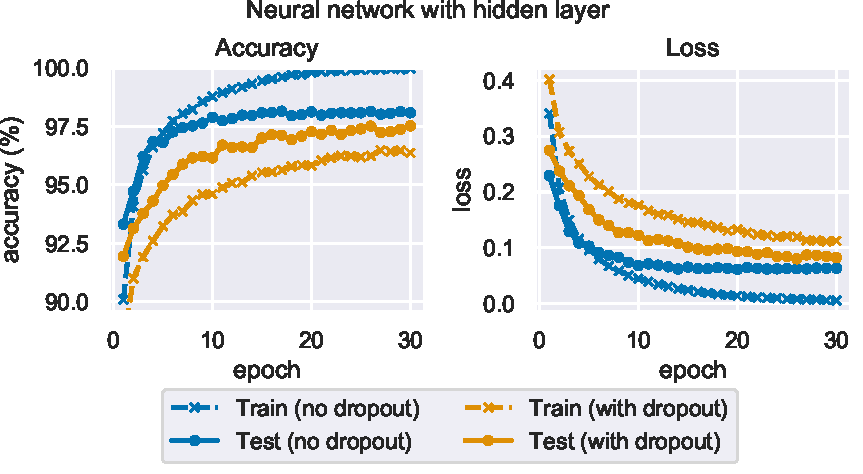
\includegraphics[scale=0.8]{fig5.pdf}
        \caption[width=7in]{
          Training the nonlinear neural network. Dropout does not measurably change test performance but prevents overfitting, at the cost of longer training time (fig5.pdf).
          \label{zfigure5}
          }
\end{figure}

\noindent \\
\begin{table}
  \centering
 \caption[width=7in]{
    Training parameters for Linear (LNN) and Nonlinear (FNN) neural networks.
    \label{ztable3}
    }
 \begin{tabular}{ccc}
 \toprule
      & Linear Neural Network & Nonlinear Neural Network \\
 \midrule
Learning Rate & 0.01 & 0.1 \\
 Decay  & 0 & 0.5 (multiplicative)\\
Momentum & 0 & 0.3 (Nesterov) \\
Batch Size & 50 & 50 \\
Number of Epochs & 7 & 30 \\
Test Set Accuracy & 90.9\% & 98.09\% \\
 \bottomrule
\end{tabular}
\end{table}

\noindent \\
\begin{figure}[H]
        \centering
        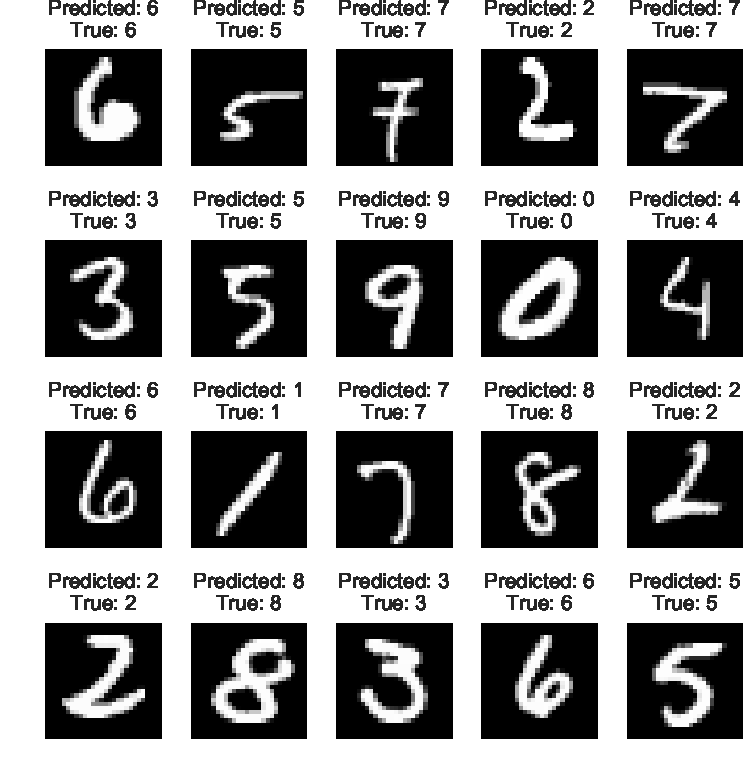
\includegraphics{fig6.pdf}
        \caption[width=7in]{Random selection of correctly classified MNIST numbers from the test set (fig6.pdf)}
        \label{zfigure6}
\end{figure}

\noindent \\
\begin{figure}[H]
        \centering
        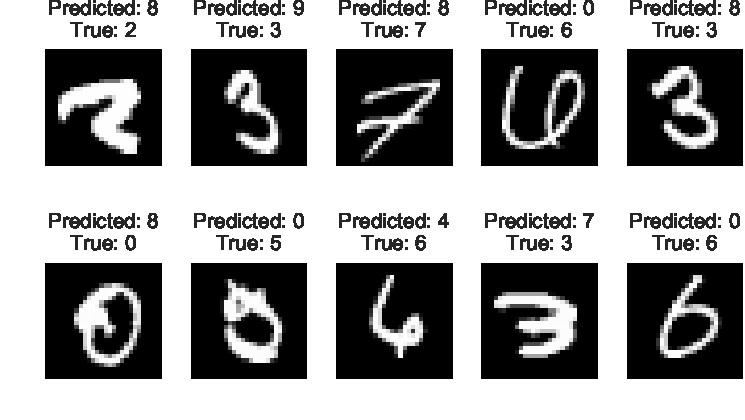
\includegraphics{fig7.pdf}
        \caption[width=7in]{Random selection of incorrectly classified MNIST numbers from the test set (fig7.pdf)}
        \label{zfigure7}
\end{figure}



\pagebreak
\begin{center}
\textbf{Part 9 }
\end{center}
\begin{biomathg}
\noindent FNN Weight Visualization
\end{biomathg}
\vspace{0.5cm}

We can visualize the mechanism of the hidden layer by plotting the weights as a grid arranged to line up with the image pixel they multiply; Figure~\ref{zfigure8} shows such an arrangement for two units from the FNN's hidden layer. (We used the network without dropout.) The unit on the left is showing what might be an edge detection in the upper left quadrant (ie. the area of darker blue - a negative weight, in contrast to the more activated red next to it). The unit on the right suggests a strong edge detection in the upper right and another activated region towards the center bottom. 

We note that the weight visualizations are dependent on the amount of training. As you increase the number of epochs the weight visualization for each unit can change significantly. For example in training with 120 epochs the weights to unit 213 were more random - more like a dead weight and the unit on the right was more strongly suggestive of a circular structure possibly the digit $0$. 

Finally we note that report included the weights to the final output nodes but we chose not to include them. We found that they did not help in terms of the interpretation of the weight visualization. In must be remembered that the bias term, amalgamation across all the weights and finally the application of the softmax will result in the final classification probabilities and this is much more complicated than just considering what if any impact the output weights contribute.

%shows very little structure. As it overlaps most digits relatively evenly, it may be picking up their total amount of lines (compare e.g. `1' and `8'). It may also be a dead unit which remains mostly ignored by the network. In contrast, the unit represented on the right shows clear circular structure which is likely suited to identify the `0` digit.

\noindent \\
\begin{figure}[H]
        \centering
        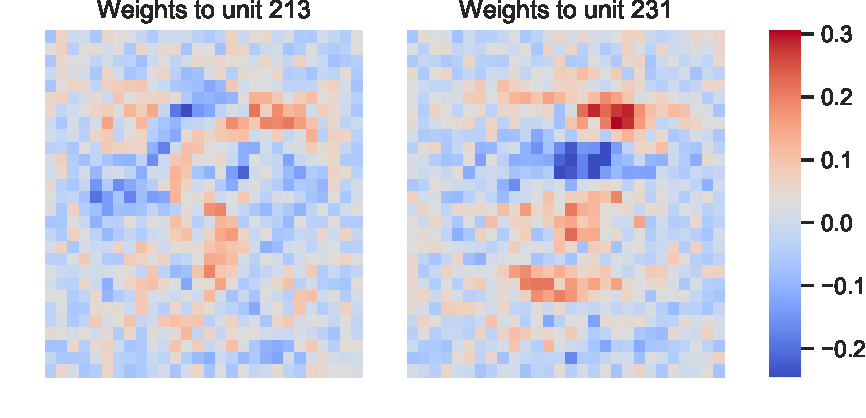
\includegraphics{fig8.pdf}
        \caption[width=7in]{
        Neural network units show a variety of structure. Shown are weights for two units from the FNN's hidden layer arranged according to which pixel of the input image they come from. Brighter colors indicate larger weights (fig9.pdf).}
        \label{zfigure8}
\end{figure}




\end{document}



























